\documentclass[../main.tex]{subfiles}
\begin{document}

\ifSubfilesClassLoaded{
	\mainmatter
	\setcounter{chapter}{5}
}{}

\chapter{Results}
\label{ch:result}
\section{Drell-Yan Cross Section Ratio}
\subsection{Results from Run 2-3 data}
\subsubsection{Effect of the updated target contamination correction}
\label{subsubsec:contamination_result}
As discussed in \cref{M-subsec:contamination}, an incorrect target contamination correction was used
in previous publications and the effect is shown in \cref{fig:contaimination_CSR}.
The overall effect is a roughly \SI{2}{\percent} shift in the ratio.
\begin{figure}[h!]
	\centering
	\includegraphics[width=0.6\linewidth]{DY-csr/Compare_targetCorr}
	\caption{The effect of the updated target contamination correction on the Drell-Y.an
		cross section. The extracted cross section ratio using the revised target contamination
		is shown as red sold triangle, and the previous published version is shown as blue open
		circle. The overall effect is a roughly \SI{2}{\percent} shift in the ratio. }
	\label{fig:contaimination_CSR}
\end{figure}



\subsubsection{Choice of fit function in intensity extrapolation}
To understand the systematic uncertainties in the intensity extrapolation method due to the
choice of fit function, the following functions are used.
\begin{align}
	R_i\left(I\right) & = p_{0i} + p_{1} I + p_{2} I^2 \quad\text{(FIT 1)}                                                     \\
	R_i\left(I\right) & = p_{0i} + \left[p_{10} + p_{11}x_i\right] I + \left[p_{20} + p_{21}x_i\right]I^2 \quad \text{(FIT 2)}
\end{align}
The fit to data using the two fits are shown in \cref{fig:run2-3_FIT1_xT,fig:run2-3_FIT2_xT}
and $\chi^2$ for the fits are tabulated in \cref{tab:chi_run23}.
And the fit for other variables are listed in \cref{M-a_ch:extrapolation}.
\begin{figure}
\centering
\caption{Fit to the flask subtracted yield ratio with FIT1 for $x_T$ for run 2-3.}
\label{fig:run2-3_FIT1_xT}
\begin{subfigure}{0.45\linewidth}
\includegraphics[width=\linewidth]{extrapolation/run2-3/xT/FIT1/hist_fitted_xT_tInt_0}
\end{subfigure}
\begin{subfigure}{0.45\linewidth}
\includegraphics[width=\linewidth]{extrapolation/run2-3/xT/FIT1/hist_fitted_xT_tInt_1}
\end{subfigure}
\begin{subfigure}{0.45\linewidth}
\includegraphics[width=\linewidth]{extrapolation/run2-3/xT/FIT1/hist_fitted_xT_tInt_2}
\end{subfigure}
\begin{subfigure}{0.45\linewidth}
\includegraphics[width=\linewidth]{extrapolation/run2-3/xT/FIT1/hist_fitted_xT_tInt_3}
\end{subfigure}
\begin{subfigure}{0.45\linewidth}
\includegraphics[width=\linewidth]{extrapolation/run2-3/xT/FIT1/hist_fitted_xT_tInt_4}
\end{subfigure}
\begin{subfigure}{0.45\linewidth}
\includegraphics[width=\linewidth]{extrapolation/run2-3/xT/FIT1/hist_fitted_xT_tInt_5}
\end{subfigure}
\end{figure}

\begin{figure}
\begin{subfigure}{0.45\linewidth}
\includegraphics{width=\linewidth}{extrapolation/run2-3/xT/FIT2/hist_fitted_xT_tInt_0}
\end{subfigure}
\begin{subfigure}{0.45\linewidth}
\includegraphics{width=\linewidth}{extrapolation/run2-3/xT/FIT2/hist_fitted_xT_tInt_1}
\end{subfigure}
\begin{subfigure}{0.45\linewidth}
\includegraphics{width=\linewidth}{extrapolation/run2-3/xT/FIT2/hist_fitted_xT_tInt_2}
\end{subfigure}
\begin{subfigure}{0.45\linewidth}
\includegraphics{width=\linewidth}{extrapolation/run2-3/xT/FIT2/hist_fitted_xT_tInt_3}
\end{subfigure}
\begin{subfigure}{0.45\linewidth}
\includegraphics{width=\linewidth}{extrapolation/run2-3/xT/FIT2/hist_fitted_xT_tInt_4}
\end{subfigure}
\begin{subfigure}{0.45\linewidth}
\includegraphics{width=\linewidth}{extrapolation/run2-3/xT/FIT2/hist_fitted_xT_tInt_5}
\end{subfigure}
\end{figure}



\Cref{fig:CSR_Run2-3} shows the extracted cross section ratio as a function of $x_T$, $x_B$ and $x_F$.
While the two fit functions produce similar results for $x_T$, the differences are slightly larger in
the other variables.

\begin{figure}[h!]
	\centering
	\begin{subfigure}{0.6\linewidth}
		\includegraphics*[width=\linewidth]{DY-csr/run23_xT}
	\end{subfigure}\\
	\begin{subfigure}{0.45\linewidth}
		\includegraphics*[width=\linewidth]{DY-csr/run23_xB}
	\end{subfigure}
	\begin{subfigure}{0.45\linewidth}
		\includegraphics*[width=\linewidth]{DY-csr/run23_xF}
	\end{subfigure}
	\caption{Comparison of the extracted Drell-Yan cross section ratio as a function of $x_T$(top),
		$x_B$(left) and $x_F$(right) using the different methods from the Run 2-3
		data.}
	\label{fig:CSR_Run2-3}
\end{figure}

\begin{table}[h!]
	\centering
	\caption{The reduced $\chi^2$ for the different fits used in the intensity extrapolation method for Run 2-3. }
	\label{tab:chi_run23}
	\begin{tabular}{|l|lll|}
\hline
 & \multicolumn{3}{c|}{$\chi^2/NDF$} \\ \cline{2-4} 
      & \multicolumn{1}{c|}{$x_T$}          & \multicolumn{1}{c|}{$x_B$}          & \multicolumn{1}{c|}{$x_F$} \\ \hline
FIT 1 & \multicolumn{1}{l|}{$40.1167 / 40$} & \multicolumn{1}{l|}{$71.3796 / 47$} & $68.0593 / 47$             \\ \hline
FIT 2 & \multicolumn{1}{l|}{$40.008 / 38$}  & \multicolumn{1}{l|}{$61.8549 / 45$} & $64.1524 / 45$             \\ \hline
\end{tabular}

\end{table}


\subsubsection{Comparison of massfit and extrapolation}
\Cref{fig:massfit_integrated_run23} shows the fit to the mass distributions for Run 2-3 data, and the
data is very well described by the fitting procedure.
\begin{figure}[h!]
	\begin{subfigure}{0.45\linewidth}
		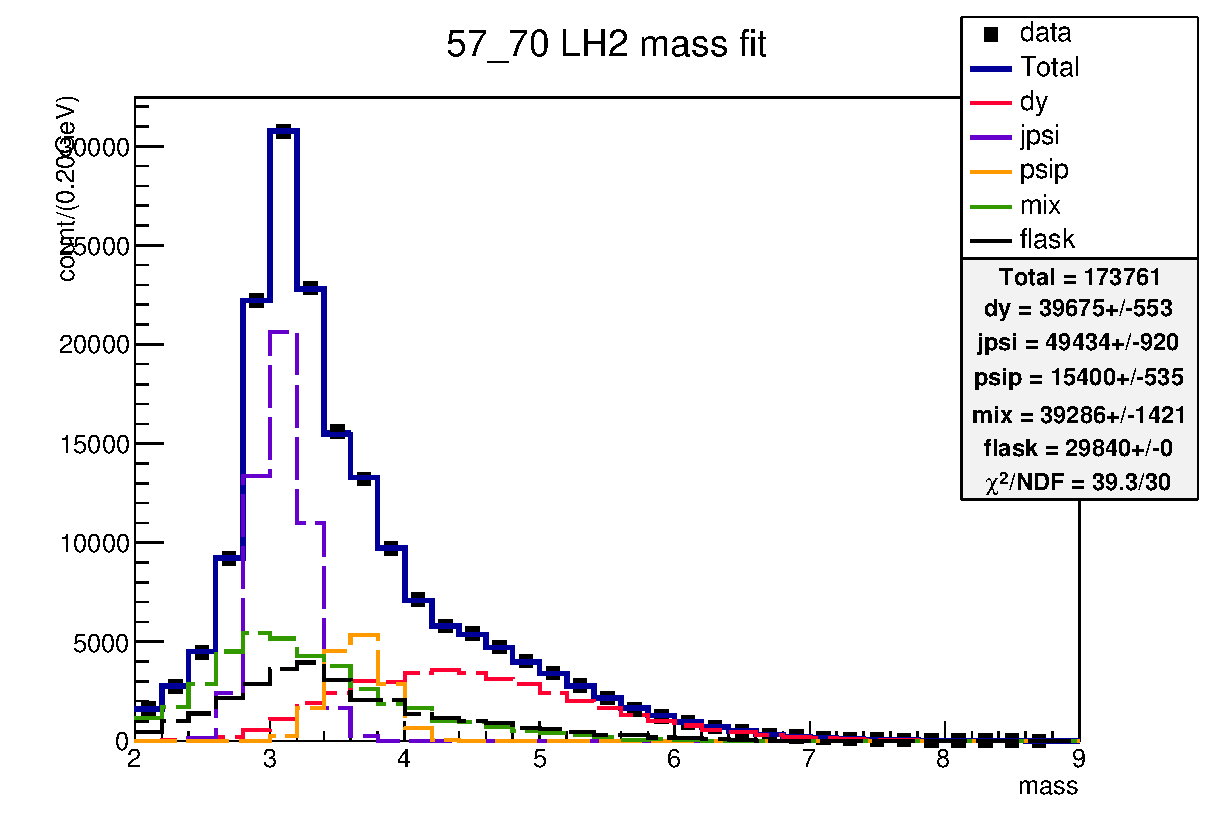
\includegraphics[width=\linewidth]{massfit/run2-3/57_70_LH2}
	\end{subfigure}
	\begin{subfigure}{0.45\linewidth}
		\includegraphics[width=\linewidth]{massfit/run2-3/57_70_LD2}
	\end{subfigure}
	\caption{The mass spectrum for \ce{LH_2}(left) and \ce{LD_2}(right) targets data for Run 2-3.}
	\label{fig:massfit_integrated_run23}
\end{figure}

With the yield for different process obtained from the mass fits, the cross section ratios can be calculated
and are also shown in \cref{fig:CSR_Run2-3}.
As reported in Ref.~\cite{dove2023} the Drell-Yan cross section ratio as a function of $x_T$ extracted from
the two methods are in very good agreement.

However, the comparison in other variables, such as $x_B$ and $x_F$ are complicated by the large
systematical uncertainties originated from the fit function used in the intensity extrapolation.
\Cref{fig:CSR_Run2-3} shows the extracted ratios as a function of $x_B$ and $x_F$ using different methods.
While the massfit results agree with the extrapolation result if FIT 1 is used, the
extrapolation results using FIT 2 are different from the other two.

\FloatBarrier

\subsection{Results from Run 5-6 data}
\Cref{fig:massfit_integrated_run56} shows the fit to the mass distributions for Run 5-6 data,
and the data is very well described by the fitting procedure.
\begin{figure}[h!]
	\begin{subfigure}{0.45\linewidth}
		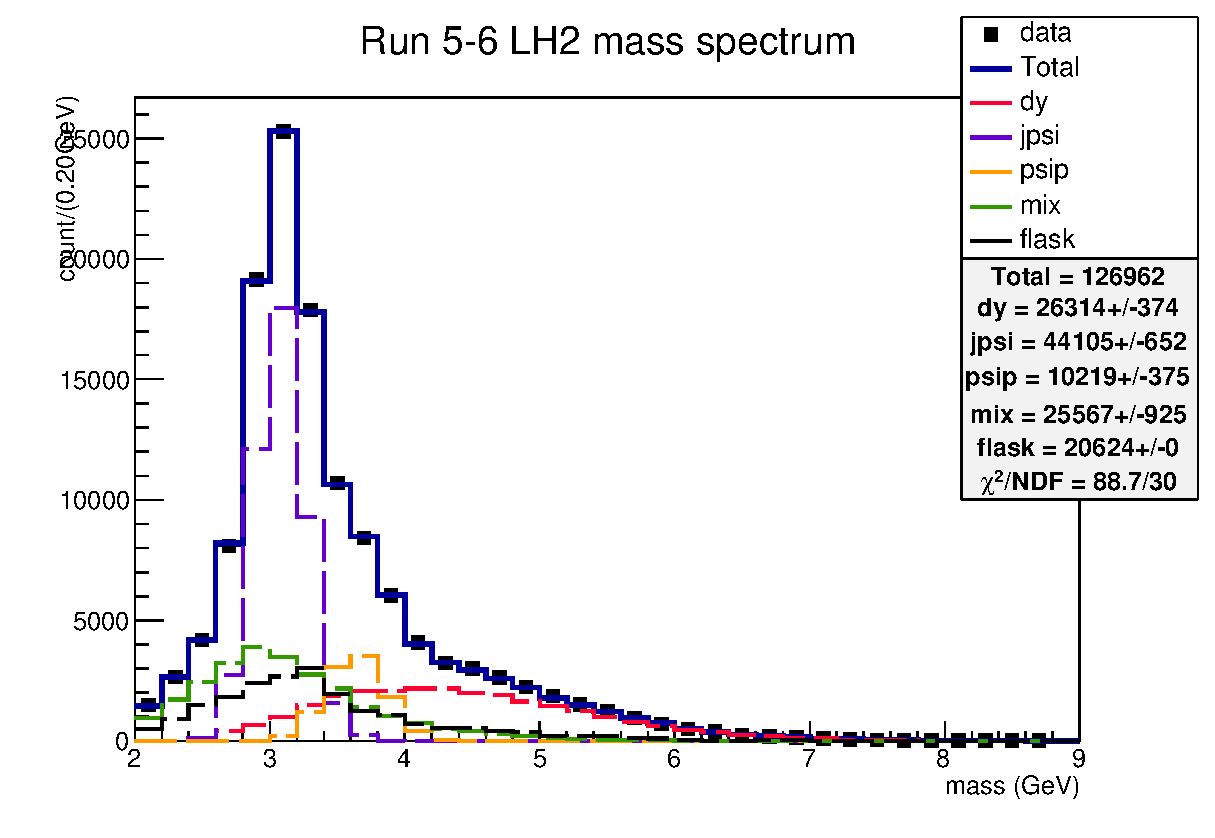
\includegraphics[width=\linewidth]{massfit/run5-6/5_6_LH2}
	\end{subfigure}
	\begin{subfigure}{0.45\linewidth}
		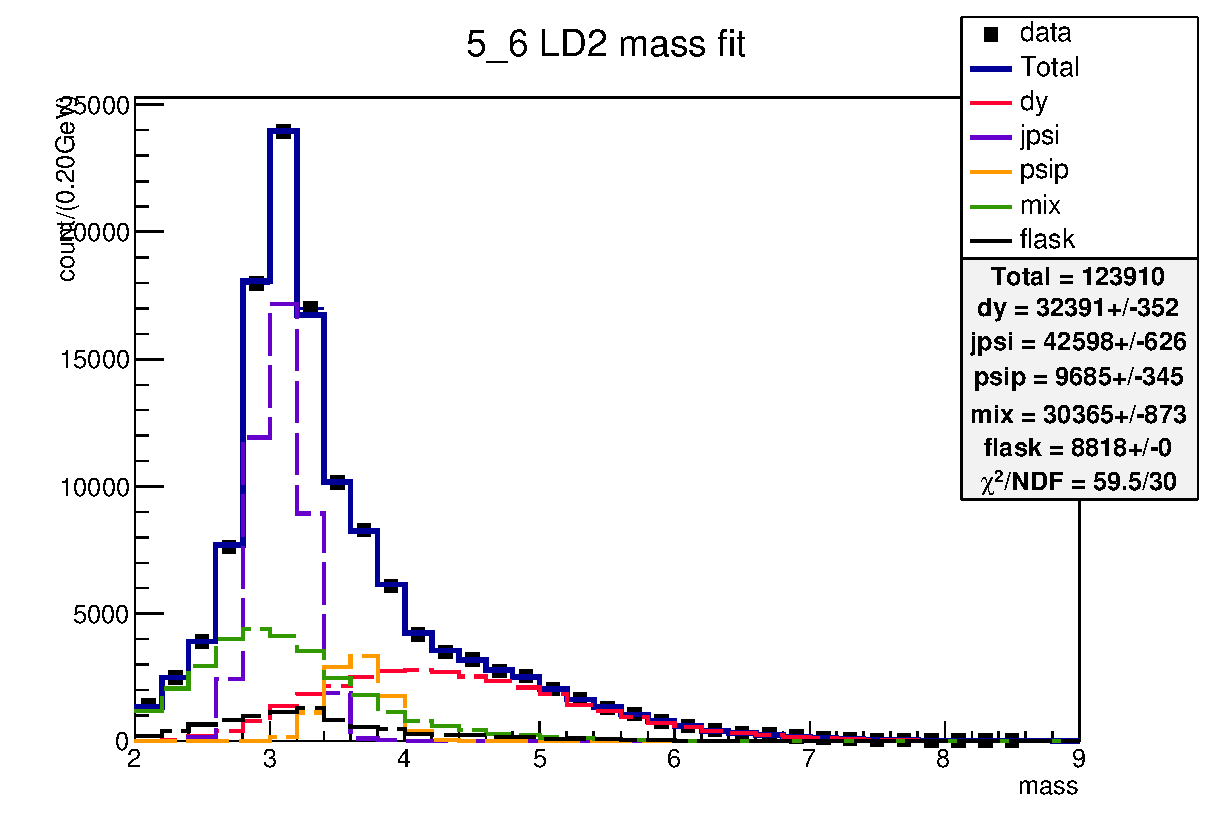
\includegraphics[width=\linewidth]{massfit/run5-6/5_6_LD2}
	\end{subfigure}
	\caption{The mass spectrum for \ce{LH_2}(left) and \ce{LD_2}(right) targets data for Run 5-6.}
	\label{fig:massfit_integrated_run56}
\end{figure}
The Drell-Yan yield for $p+p$ and $p+d$ can then be extracted and the cross section ratios
are shown in \cref{fig:CSR_Run5-6}.

To extract the cross section ratio using the intensity extrapolation method, the yield ratios
calculated as function of $x_T$ and intensity and the fits are shown in \cref{fig:run5-6_FIT1_xT}
(FIT 1) and \cref{fig:run5-6_FIT2_xT} (FIT 2), with the fits for other variables listed in
\cref{M-a_ch:extrapolation}. And the reduced $\chi^2$ is tabulated in \cref{tab:chi_run56}.
\begin{figure}
	\centering
	\caption{Fit to the flask subtracted yield ratio with FIT1 for $x_T$ for run 5-6.}
	\label{fig:run5-6_FIT1_xT}
	\begin{subfigure}{0.45\linewidth}
		\includegraphics[width=\linewidth]{extrapolation/run5-6/xT/FIT1/hist_fitted_xT_tInt_0}
	\end{subfigure}
	\begin{subfigure}{0.45\linewidth}
		\includegraphics[width=\linewidth]{extrapolation/run5-6/xT/FIT1/hist_fitted_xT_tInt_1}
	\end{subfigure}
	\begin{subfigure}{0.45\linewidth}
		\includegraphics[width=\linewidth]{extrapolation/run5-6/xT/FIT1/hist_fitted_xT_tInt_2}
	\end{subfigure}
	\begin{subfigure}{0.45\linewidth}
		\includegraphics[width=\linewidth]{extrapolation/run5-6/xT/FIT1/hist_fitted_xT_tInt_3}
	\end{subfigure}
	\begin{subfigure}{0.45\linewidth}
		\includegraphics[width=\linewidth]{extrapolation/run5-6/xT/FIT1/hist_fitted_xT_tInt_4}
	\end{subfigure}
	\begin{subfigure}{0.45\linewidth}
		\includegraphics[width=\linewidth]{extrapolation/run5-6/xT/FIT1/hist_fitted_xT_tInt_5}
	\end{subfigure}
\end{figure}

\input{section/extrapolation_xT_56_2.tex}
From the fits, the cross section ratio can be extracted.

\pdfmargincomment{run 5-6 compared with 2-3 and full data set, only show massfit results?}
\Cref{fig:CSR_Run5-6} shows the extracted cross section ratio as a function from the
second half of our data using various methods. While the different fit functions used in the
intensity extrapolation produce very similar results, the massfit result is significantly larger
than the intensity extrapolation results. This difference is included in the systematic uncertainties
for the final Drell-Yan cross section ratio from Run 5-6.
\begin{figure}[h!]
	\centering
	\begin{subfigure}{0.6\linewidth}
		\includegraphics*[width=\linewidth]{DY-csr/run56_xT}
	\end{subfigure}
	\begin{subfigure}{0.45\linewidth}
		\includegraphics*[width=\linewidth]{DY-csr/run56_xB}
	\end{subfigure}
	\begin{subfigure}{0.45\linewidth}
		\includegraphics*[width=\linewidth]{DY-csr/run56_xF}
	\end{subfigure}
	\caption{Comparison of the extracted Drell-Yan cross section ratio as a function of $x_T$(top),  $x_B$(left)
		and $x_F$(right) from the Run 5-6 data using the massfit and intensity extrapolation method.}
	\label{fig:CSR_Run5-6}
\end{figure}
\begin{table}
	\centering
	\caption{The reduced $\chi^2$ for the different fits used in the intensity extrapolation method for Run 5-6. }
	\label{tab:chi_run56}
	\begin{tabular}{|l|lll|}
\hline
 & \multicolumn{3}{c|}{$\chi^2/NDF$} \\ \cline{2-4} 
      & \multicolumn{1}{c|}{$x_T$}          & \multicolumn{1}{c|}{$x_B$}          & \multicolumn{1}{c|}{$x_F$} \\ \hline
FIT 1 & \multicolumn{1}{l|}{$24.3236 / 28$} & \multicolumn{1}{l|}{$41.6412 / 33$} & $28.1757 / 33$             \\ \hline
FIT 2 & \multicolumn{1}{l|}{$23.2091 / 26$}  & \multicolumn{1}{l|}{$40.3455 / 31$} & $25.7949 / 31$             \\ \hline
\end{tabular}

\end{table}

\subsubsection{Potential cause of difference between massfit and intensity extrapolation}
During the second half of the data taking, the variation in the instantaneous beam
intensity was reduced as compared to run 2-3. This is partly due to the improvement
in beam quality and partly due to the tightening of the beam inhibit thresholds.

The massfit and intensity extrapolation methods made different assumption on the intensity
and rate dependence. With less high intensity data, there are less constraints on the
intensity dependence, causing the two method to disagree.

\pdfcomment{Intensity range cannot explain the discrepancy }
\Cref{fig:CSR_combined} shows the final results from the two datasets. The two datasets
are consistent with each other, partly due to the large systematic uncertainties in the
Run 5-6 results, which is dominated by the differences between the massfit and intensity
extrapolation methods.
\begin{figure}
	\centering
	\begin{subfigure}{0.6\linewidth}
		\includegraphics*[width=\linewidth]{DY-csr/method_full_xT_syst}
	\end{subfigure}
	\begin{subfigure}{0.45\linewidth}
		\includegraphics[width=\linewidth]{DY-csr/method_full_xB_syst}
	\end{subfigure}
	\begin{subfigure}{0.45\linewidth}
		\includegraphics[width=\linewidth]{DY-csr/method_full_xF_syst}
	\end{subfigure}
	\caption{Comparison of the extracted Drell-Yan cross section ratio as a function of $x_T$(top),  $x_B$(left)
		and $x_F$(right) from the two datasets.}
	\label{fig:CSR_combined}
\end{figure}


\subsection{Comparison with global PDF analysis}
\pdfmargincomment{modified to impact of SeaQuest result?}
The published $\sigma_{pd}/2\sigma_{pp}$ ratio result has been included in various recent global
PDF analysis, including Ref.~\cite{cocuzza2021,guzzi2022,accardi2023,alekhin2023}.
In particular, \cref{fig:CSR_Run2-3} shows the calculation using CT18 (without the SeaQuest data)
and NNPDF 4.0 (including the SeaQuest data). The shift in the cross section ratio is primarily
coming from the inclusion of the SeaQuest data. Unlike the previous E866 result, the SeaQuest data
strongly suggests the $\bar{d}/\bar{u}$ ratio would remain greater than one for $x<0.4$, which is
consistent with prediction from various models, including meson cloud and statistical model.

The importance of the SeaQuest data can be seen in the NNPDF 4.0, where at large $x_T$,
uncertainties bands is consistent with the uncertainties of our measurements, as the SeaQuest
results is the only available data sensitive to the light sea-quark asymmetry at large $x$.
\FloatBarrier
\subfile{4_2_result_jpsi}

\ifSubfilesClassLoaded{ \printbibliography[heading=bibintoc,title={References}]}{}

\end{document}
